\section{主题聚合与价值评估结果}

人工确认结果中 100 条机会记录进入语义聚合。使用 384 维多语言 E5 向量和 HDBSCAN，距离度量为欧氏距离，参数为 $\text{min\_cluster\_size}=5$、$\text{min\_samples}=2$。聚类得到 14 个主题，12 个主题只有一条记录，12 条噪声记录按单记录主题保留；轮廓系数在非噪声成员上计算，为 0.204。图~\ref{fig:topicscore} 对比各主题的成员规模与价值分，显示结果由两个较大的主题和 12 个单记录主题构成。

主题稀疏说明人工确认机会中仍有较多具体而分散的需求，不能把每个主题都视为成熟市场方向。排序第一的主题为 C2，价值分为 85.76，成员来自 GitHub、V2EX 和量子位；但该主题同时包含 AI 信息整理、游戏、医疗协同、Agent 平台和工具介绍等内容，主题内部异质性明显。因此 C2 在本文中仅作为系统发现的高分候选和聚类局限示例，不被解释为单一可立即立项的产品方向。

\begin{figure}[H]
  \centering
  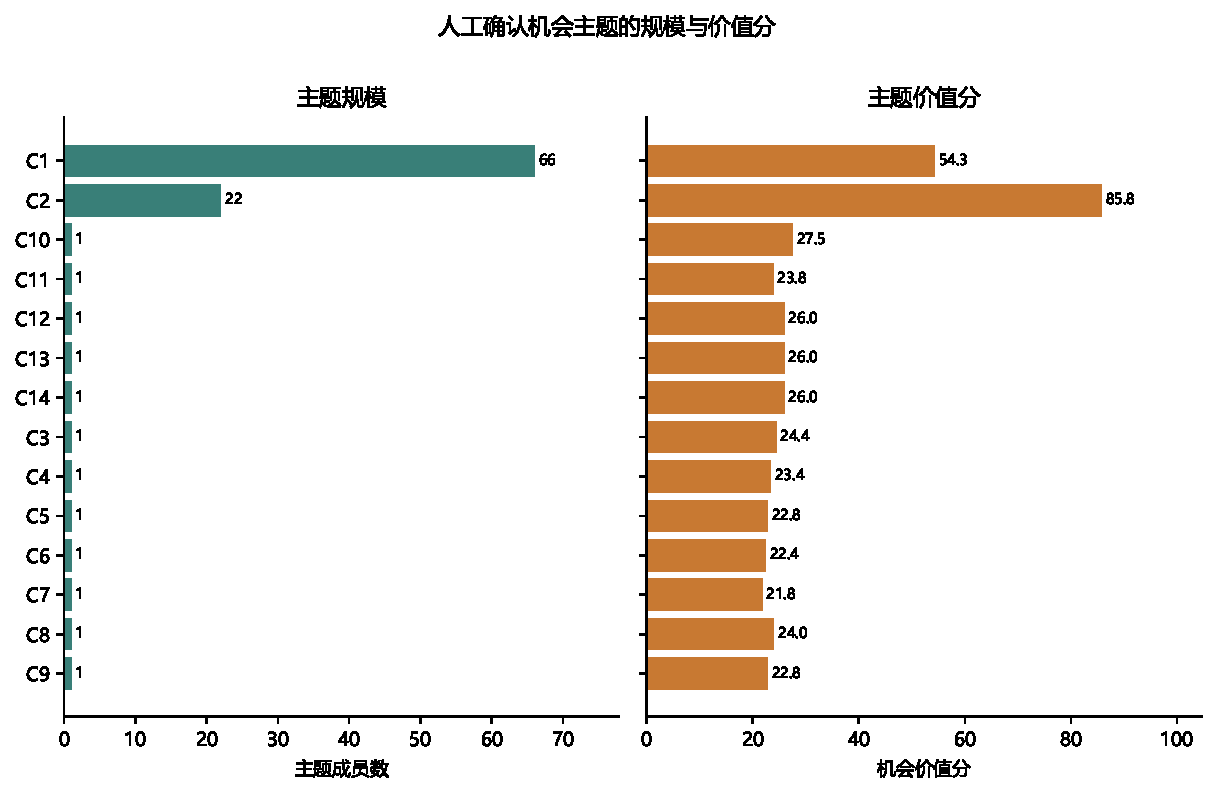
\includegraphics[width=0.95\textwidth]{../figures/fig05_topic_size_score.pdf}
  \caption{人工确认机会主题的成员规模与价值分。大多数主题为单记录主题，C1 和 C2 的规模明显高于其余主题。}
  \label{fig:topicscore}
\end{figure}

价值评分使用多源指向度、记录规模和互动信号三项维度，权重分别为 0.45、0.35 和 0.20。权重扰动下，来源、规模和互动信号情景与基准排序的 Kendall 相关系数分别为 1.000、1.000 和 1.000。由于主题数量较少且大量主题为单记录，该结果只能说明当前候选样本中的排序对权重变化不敏感，不能说明排序具有外部有效性；敏感性分析没有覆盖机会标签和聚类参数的变化。

图~\ref{fig:topic-dimensions} 将每个主题的三个维度分别展示，互动信号缺失的主题单独留空。C2 的跨来源覆盖与互动信号得分较高，C1 则主要依靠记录规模维度；这使得总分能够分解回已取得的数据字段，但仍受人工复核样本和平台覆盖偏差影响。

\begin{table}[H]
  \centering
  \caption{两个多记录主题的价值评分构成}
  \label{tab:topic-scores}
  \begin{tabular}{lrrrrr}
    \toprule
    主题 & 记录数 & 网站数 & $S_c$ & $N_c$ & $H_c$ / 总分 \\
    \midrule
    C2 智能体多场景应用 & 22 & 3 & 100.00 & 74.57 & 73.30 / 85.76 \\
    C1 AI 编程助手工作流 & 66 & 1 & 33.33 & 100.00 & 21.32 / 54.26 \\
    \bottomrule
  \end{tabular}
\end{table}

C2 的高分主要来自 3 个网站覆盖和较强的互动信号；C1 虽然包含 66 条记录，却全部来自 Hacker News，跨来源维度较低。该对比说明评分会把来源多样性纳入排序，但不同来源并不等于独立需求，仍需回到来源事件和成员文本判断重复传播及真实问题。

\begin{figure}[H]
  \centering
  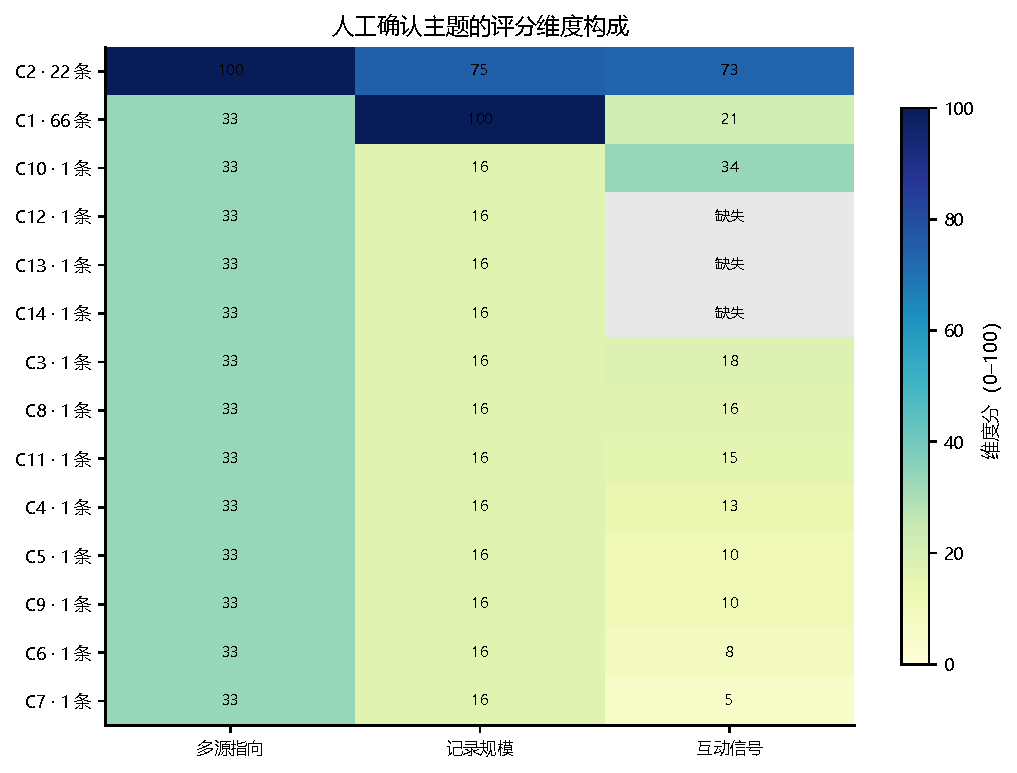
\includegraphics[width=0.77\textwidth]{../figures/fig13_topic_dimension_heatmap.pdf}
  \caption{14 个人工确认机会主题的多源指向度、记录规模和互动信号得分。互动信号缺失以空格显示，维度分仅用于当前 B01 候选排序。}
  \label{fig:topic-dimensions}
\end{figure}

为观察连续改变权重对排序的影响，图~\ref{fig:topic-rank-sensitivity} 从对称 Dirichlet$(1,1,1)$ 分布抽取 20,000 组权重，并对可用维度重新归一。点和误差线分别表示排名中位数及第 10--90 百分位，标签中的“前三”表示主题进入前三名的抽样比例。在这一权重先验下，C2 均保持前三，C1 有 91\% 的权重抽样进入前三。该比例描述指定权重扰动下的计算频率，不是主题真实优先级的概率；样本和机会标签的不确定性未包含在此模拟中。

\begin{figure}[H]
  \centering
  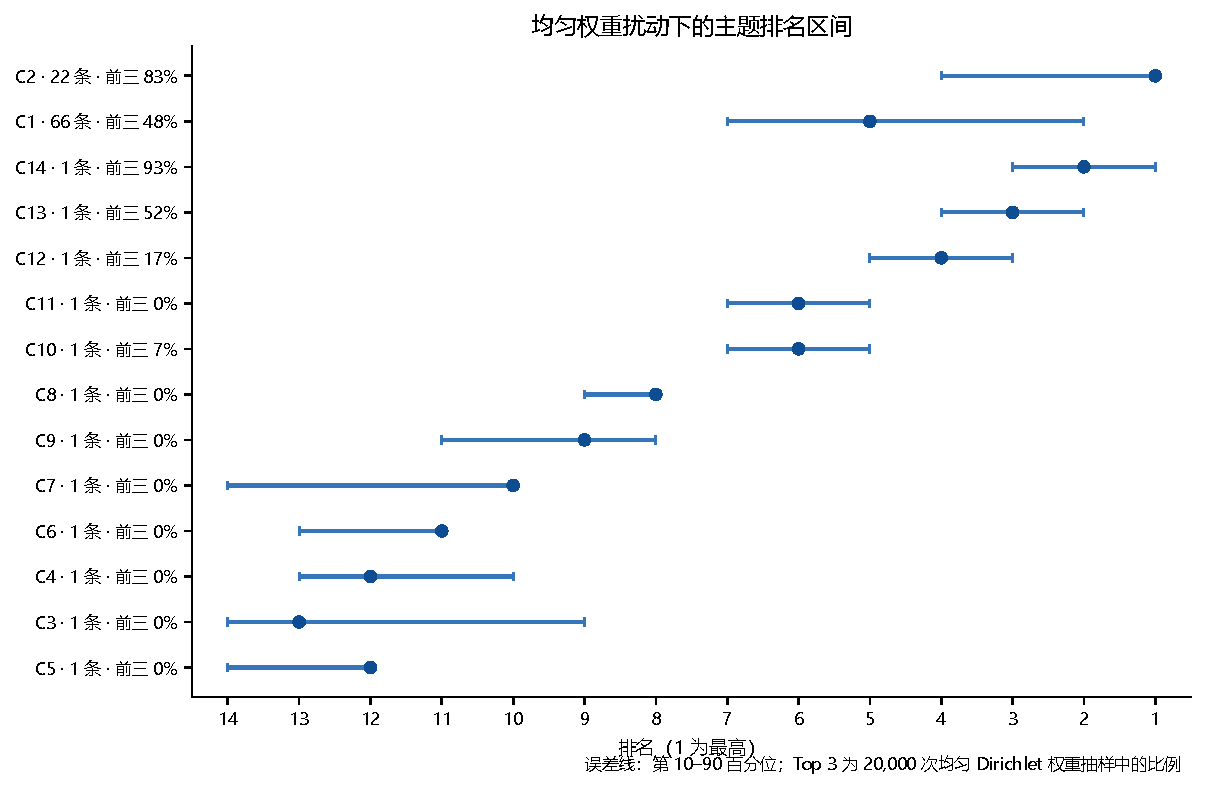
\includegraphics[width=0.86\textwidth]{../figures/fig14_topic_rank_sensitivity.pdf}
  \caption{人工确认主题在 20,000 组等先验权重抽样下的排名区间。误差线为第 10--90 百分位，“前三”比例只描述指定权重分布，不构成主题外部有效性证据。}
  \label{fig:topic-rank-sensitivity}
\end{figure}
